%%%%%%%%%%%%%%%%%%%%%%%%%%%%%%%%%%%%%%%%%%%%%%%%%%%%%%%%%%%%%%%%%%%%
%% I, the copyright holder of this work, release this work into the
%% public domain. This applies worldwide. In some countries this may
%% not be legally possible; if so: I grant anyone the right to use
%% this work for any purpose, without any conditions, unless such
%% conditions are required by law.
%%%%%%%%%%%%%%%%%%%%%%%%%%%%%%%%%%%%%%%%%%%%%%%%%%%%%%%%%%%%%%%%%%%%

\documentclass{beamer}

\logo{\includesvg[width=3cm]{HorizontalStacked_RGB.svg}}

\usetheme[faculty=fi]{fibeamer}
\usepackage[utf8]{inputenc}
\usepackage[main=english]{babel}
%%
%% These macros specify information about the presentation
\title{Deep Learning in R} %% that will be typeset on the
\subtitle{Application in Image Analysis} %% title page.
\author{Robert E. Settlage, PhD, MS \newline Nov 2018}
%% These additional packages are used within the document:
\usepackage{ragged2e}  % justifying text
\usepackage{booktabs}  % Tables
\usepackage{tabularx}
\usepackage{tikz}      % Diagrams
\usetikzlibrary{calc, shapes, backgrounds}
\usepackage{amsmath, amssymb}
\usepackage{url}       % urls
\usepackage{listings}  % Code listings
\usepackage{svg}
\usetikzlibrary{matrix}
\usetikzlibrary{positioning}
\usetikzlibrary{backgrounds}
\usepackage{minted}
\usepackage{alltt}

%%%%%%%%%%%%%%%%%%% Local functions %%%%%%%%%%%%%%%%%%%
%% -- Draw marks
\newbox\dumbox
\newcommand{\mymark}[2]{%
  \setbox\dumbox=\hbox{#2}%
  \hbox to \wd\dumbox{\hss%
    \tikz[overlay,remember picture,baseline=(#1.base)]{ \node (#1) {\box\dumbox}; }%
    \hss}%
}

%% -- Draw small coefficient
\newcommand{\mysmall}[1]{%
  \tikz[overlay,remember picture]{%
    \node[blue,scale=.5, shift={(0,-.1)}] {x#1};%
  }%
}
%%%%%%%%%%%%%%%%%%% Local functions %%%%%%%%%%%%%%%%%%%



\begin{document}
  \frame{\maketitle}
  \begin{darkframes}
    \small
    \begin{frame}[label=lists]{Goals and Objectives}
    \framesubtitle{Give R a little love}
      \begin{itemize}
          \item Introduce ARC at VT
          \item Introduce concepts of Deep Learning for image analysis
          \item Walk-through image analysis in R
      \end{itemize}
          
    \end{frame}

    \begin{frame}{Advanced Research Computing}
      \framesubtitle{Virginia Tech}
      \begin{block}
      {\small{Unit within the Office of the Vice President of Information Technology.}}
      Goal: Further research by lowering barriers to the use of HPC and Viz
      \end{block}
      \begin{columns}[onlytextwidth]
      \column{0.65\textwidth}
      \begin{itemize}
          \item Centralize resource acquisition, maintenance, and support for research community
          \item Provide support to facilitate usage of resources and minimize barriers to entry
          \item Enable and participate in research collaborations between departments
      \end{itemize}
      \column{0.3\textwidth}
      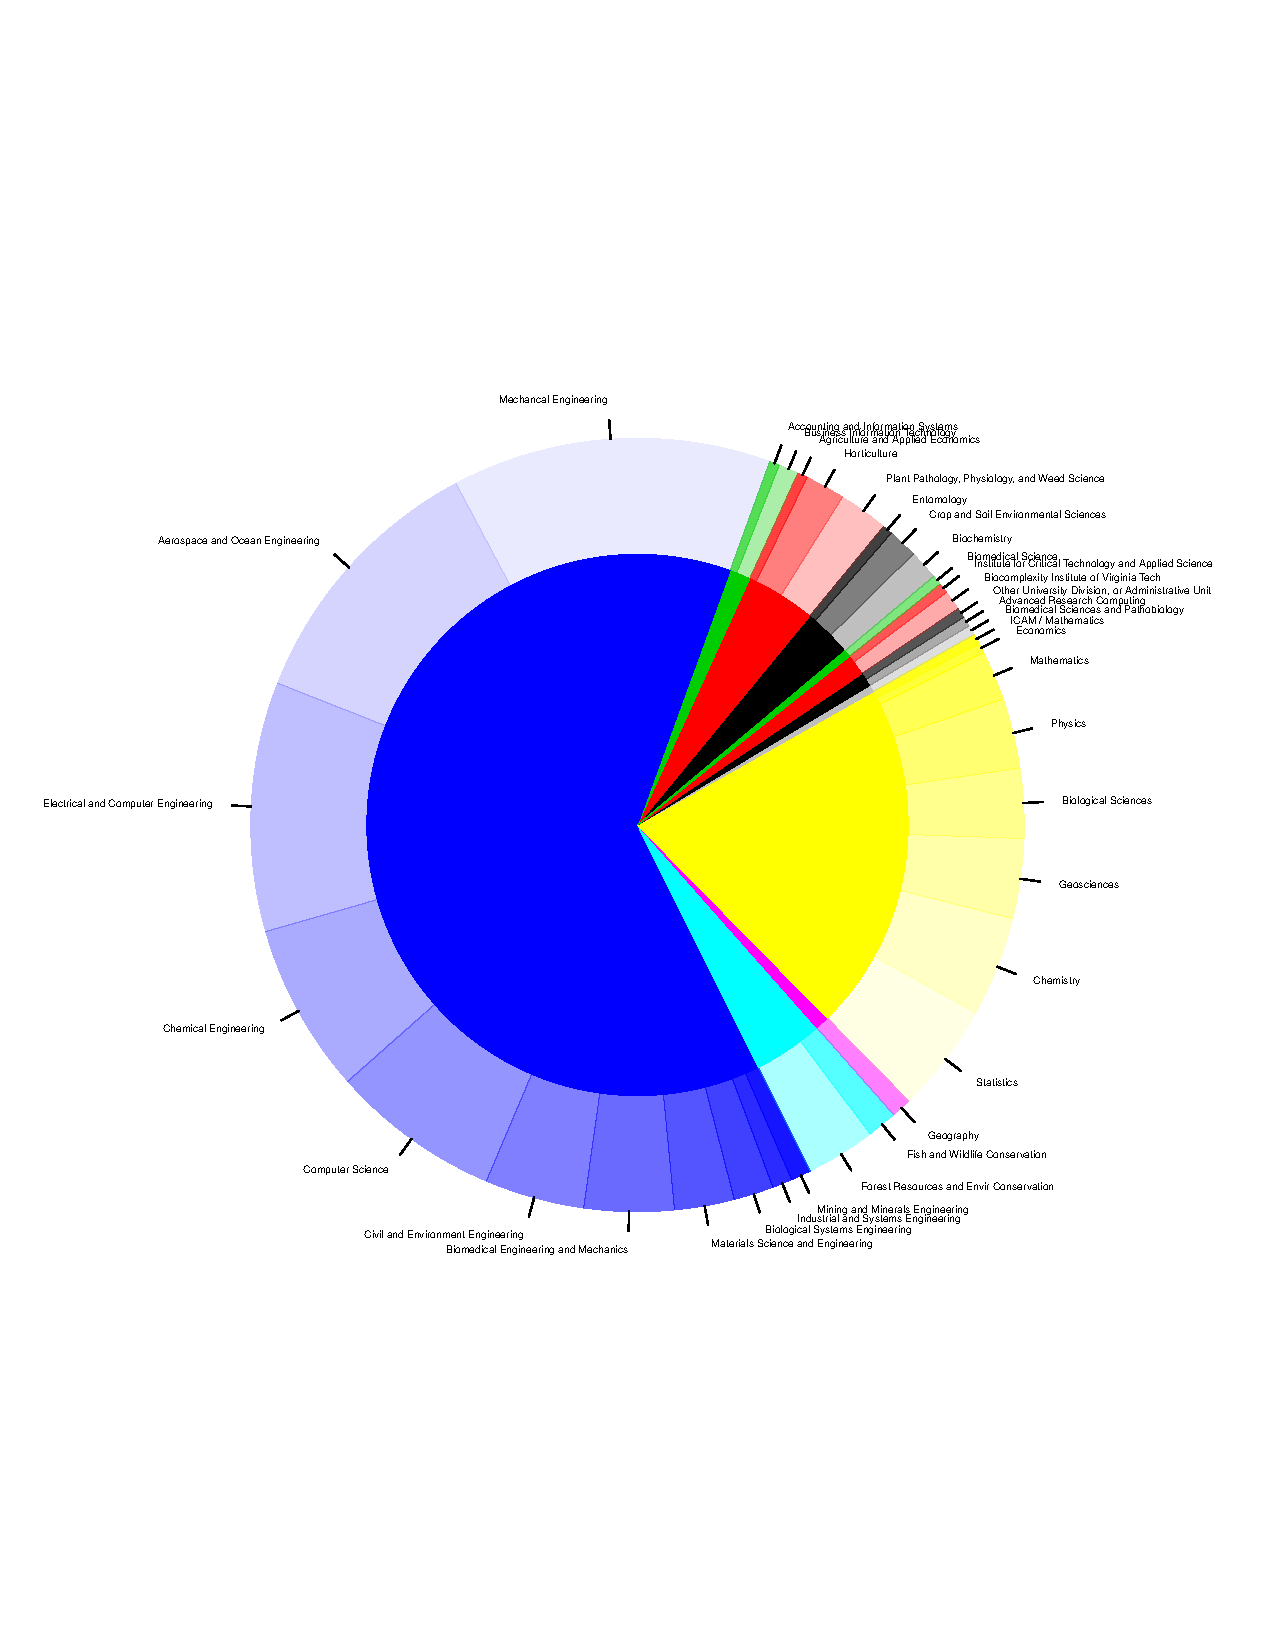
\includegraphics[width=3cm]{College_usage.pdf}
      \end{columns}
    \end{frame}
    
    \begin{frame}{Deep Learning}
      \framesubtitle{Basic concepts}
      \begin{block}
      {data + compute + algorithms}
        An abundance of data (labeled), computing power (GPUs), and algorithm developments in CS, statistics, math etc have led to a revolution in automated feature discovery and model building/optimization.
      \end{block}
      \bigskip
        % Generic DL algorithm
        \tikzstyle{startstop} = [rectangle, rounded corners, minimum width=2cm, minimum height=1cm,text centered, draw=black, fill=black!40]
        \tikzstyle{arrow} = [thick,->,>=stealth]
        \tikzstyle{process} = [rectangle, rounded corners, minimum width=2cm, minimum height=1cm, text centered, draw=black, fill=black!40]
        \begin{tikzpicture}
        \node (Data) [startstop] {Data};
        \node (Model) [process, right of=Data, xshift=2cm] {Model};
        \node (Scoring) [process, right of=Model, xshift=2cm] {Scoring};
        \node (Refine) [process, below of=Scoring, yshift=-0.5cm] {Propogate};
        \draw [arrow] (Data) -- (Model);
        \draw [arrow] (Model) -- (Scoring);
        \draw [arrow] (Scoring) -- (Refine);
        \draw [arrow] (Refine) -| (Model);
        \end{tikzpicture}
      
    \end{frame}
    
    
    \begin{frame}{Deep Learning}
      \framesubtitle{Image analysis -- data}
      \begin{block}
      {\small{Key features:}}
      \begin{itemize}
          \item Lots of labelled data
          \item As Cassie Kozyrkov says, “Split your damn data”.  Train/Validate/Test
      \end{itemize}
      \end{block}
      \bigskip
      \begin{block}
      {\small{Process:}}
      \begin{itemize}
          \item All data is processed identically.
          \item Images should be standardized.
      \end{itemize}
      \end{block}
    \end{frame}
    
    \begin{frame}{Deep Learning}
      \framesubtitle{Feature discovery -- convolutional neural networks}
      \begin{block}
      {\small{At the crux of deep learning in image processing are convolutions.}}
      Feature discovery through sliding matrix operations. 
      \end{block}

      \begin{columns}[onlytextwidth]
        \column{.4\textwidth}
            \begin{table}[]
            \begin{tabular}{llllll}
            0 & 0 & \textcolor{red}{0} & \textcolor{red}{3} & \textcolor{red}{0} & 0 \\
            0 & 0 & \textcolor{red}{7} & \textcolor{red}{0} & \textcolor{red}{4} & 0 \\
            0 & 0 & \textcolor{red}{2} & \textcolor{red}{0} & \textcolor{red}{4} & 0 \\
            0 & 0 & 0 & 6 & 0 & 0 \\
            0 & 0 & 0 & 0 & 0 & 0
            \end{tabular}
            \end{table}
        \column{.3\textwidth}
            \begin{table}[]
            \begin{tabular}{lll}
            0 & 0 & 0 \\
            1 & 1 & 1 \\
            0 & 0 & 0
            \end{tabular}
            \end{table}
        \column{.3\textwidth}
            \begin{table}[]
            \begin{tabular}{llll}
            7 & 7 & \textcolor{orange}{11} & 4 \\
            2 & 2 & 6 & 4 \\
            0 & 6 & 6 & 6 
            \end{tabular}
            \end{table}
      \end{columns}
        
    \end{frame}
    
        \begin{frame}{Deep Learning}
      \framesubtitle{Convolutional neural networks -- convolutions}
      \begin{block}
      {\small{Convolutions are filters.}}
      Edge detector visualized. 
      \end{block}
      \begin{center}
      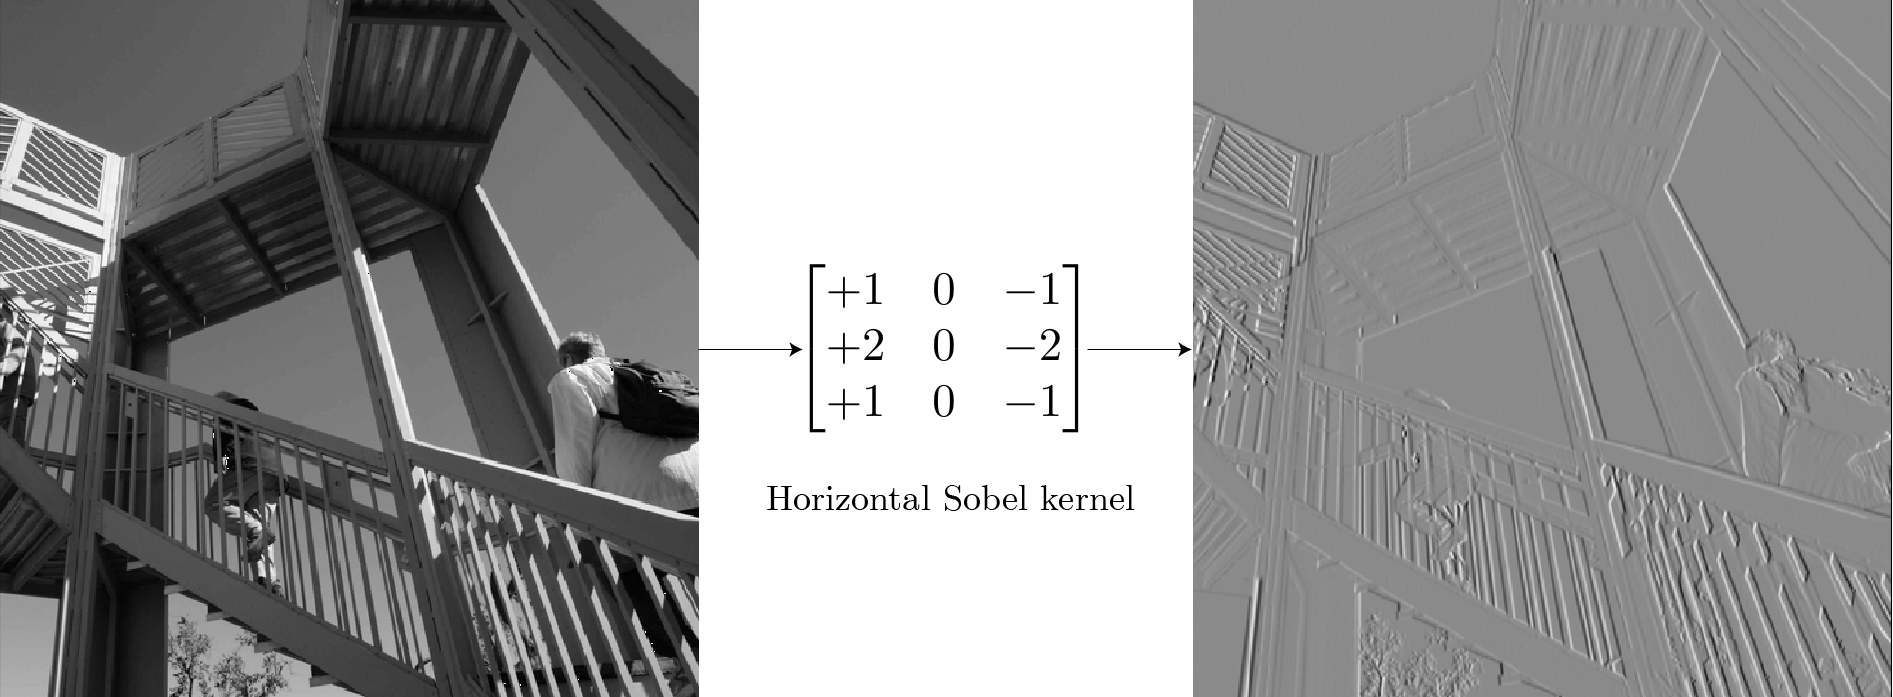
\includegraphics[width=9cm]{sobel_kernel.png}  \\
      \tiny{towardsdatascience.com/intuitively-understanding-convolutions-for-deep-learning}
      \end{center}
    \end{frame}
    
    \begin{frame}{Deep Learning}
      \framesubtitle{Convolutional neural networks -- CNNs}
      \begin{block}
      {\small{Convolutions are combined in an artificial neural network to construct the basis for feature extraction and combination to build a model.}}
      \end{block}
      
       % Generic CNN algorithm
        \def\layersep{2.5cm}
        
        \begin{tikzpicture}[
           shorten >=1pt,->,
           draw=black!50,
            node distance=\layersep,
            every pin edge/.style={<-,shorten <=1pt},
            neuron/.style={circle,fill=black!25,minimum size=12pt,inner sep=0pt},
            input neuron/.style={neuron, fill=green!50},
            output neuron/.style={neuron, fill=red!50},
            hidden neuron/.style={neuron, fill=blue!50},
            annot/.style={text width=4em, text centered}]
            
            % Draw the input layer nodes
            \foreach \name  [count=\y] in 
            {Pixel 1, Pixel 2, Pixel 3}
             {   \node[input neuron, pin=left:\name] (I-\y) at (0,-\y cm) {};  
             }
        
            % set number of hidden layers
            \newcommand\Nhidden{2}
            \newcommand\NodOne{4}
            \newcommand\NodTwo{5}
            \newcommand\Nod{3}
        
            % Draw the hidden layer nodes
             \foreach \y in {1,...,\NodOne} {
                  \path[yshift=0.5cm]
                      node[hidden neuron] (H1-\y) at (1*\layersep,-\y cm) {};
                      }
            \node[annot,above of=H1-1, node distance=1cm] (hl1) {Hidden layer 1};
             \foreach \y in {1,...,\NodTwo} {
                  \path[yshift=0.5cm]
                      node[hidden neuron] (H2-\y) at (2*\layersep,-\y cm) {};            
                   }
            \node[annot,above of=H2-1, node distance=1cm] (hl2) {Hidden layer 2};          
        
            % Draw the output layer node
            \node[output neuron,pin={[pin edge={->}]right:cat?}, right of=H\Nhidden-3] (O) {};
        
            % Connect every node in the input layer with every node in the
            % hidden layer.
            \foreach \source in {1,...,3}{
                \foreach \dest in {1,...,\NodOne}{
                    \path (I-\source) edge (H1-\dest);
                 }
            }
            % connect all hidden stuff
            \foreach [remember=\N as \lastN (initially 1)] \N in {2,...,\Nhidden}
               \foreach \source in {1,...,\NodOne}
                   \foreach \dest in {1,...,\NodTwo}
                       \path (H\lastN-\source) edge (H\N-\dest);
        
            % Connect every node in the hidden layer with the output layer
            \foreach \source in {1,...,\NodTwo}
                \path (H\Nhidden-\source) edge (O);
        
            % Annotate the layers
        
            \node[annot,left of=hl1] {Input layer};
            \node[annot,right of=hl\Nhidden] {Output layer};
        \end{tikzpicture}
        
    \end{frame}
    
    \begin{frame}{Deep Learning}
      \framesubtitle{Scoring and learning}
      \begin{block}
      {\small{Scoring: How well did the model work?}}
      \begin{itemize}
          \item Lots of labelled data
          \item Some measure of how well the model fit.  $L_2$ loss?
      \end{itemize}
      \end{block}
      \smallskip
      \begin{block}
      {\small{Learning:  Data $\xrightarrow{}$ Model $\xrightarrow{}$ Score $\xrightarrow{}$ Improve.}}
      \begin{itemize}
          \item This is an optimization problem.  Given data, what params give best fit.
          \item Gradient descent and "back-propogate" to get improvement.  
      \end{itemize}
      \end{block}
    \end{frame}
    
    \begin{frame}{Deep Learning}
      \framesubtitle{Basic concepts}
      \begin{block}
      {data + compute + algorithms}
        An abundance of data (labeled), computing power (GPUs), and algorithm developments in CS, statistics, math etc have led to a revolution in automated feature discovery and model building/optimization.
      \end{block}
      \bigskip
        % Generic DL algorithm
        \tikzstyle{startstop} = [rectangle, rounded corners, minimum width=2cm, minimum height=1cm,text centered, draw=black, fill=black!40]
        \tikzstyle{arrow} = [thick,->,>=stealth]
        \tikzstyle{process} = [rectangle, rounded corners, minimum width=2cm, minimum height=1cm, text centered, draw=black, fill=black!40]
        \begin{tikzpicture}
        \node (Data) [startstop] {Data};
        \node (Model) [process, right of=Data, xshift=2cm] {Model};
        \node (Scoring) [process, right of=Model, xshift=2cm] {Scoring};
        \node (Refine) [process, below of=Scoring, yshift=-0.5cm] {Propogate};
        \draw [arrow] (Data) -- (Model);
        \draw [arrow] (Model) -- (Scoring);
        \draw [arrow] (Scoring) -- (Refine);
        \draw [arrow] (Refine) -| (Model);
        \end{tikzpicture}
      
    \end{frame}
    
    \begin{frame}{R}
      \framesubtitle{mature open-source scripting language for statistical analysis}
      \begin{block}
      {\small{Developed by statisticians and has excellent graphics system.}}
      \end{block}
      \bigskip
      \begin{itemize}
          \item extensive base and user developed libraries
          \item ability to hand-off to compiled languages, e.g. Fortran, C++, CUDA
          \item ability to harness computing power offered by GPU devices
      \end{itemize}
    \end{frame}
    
        \begin{frame}{R - Keras}
      \begin{block}
      {\small{Keras sits on top of TensorFlow and abstracts the TF interface.}}
      \begin{itemize}
          \item RNN, LTSTM, CNN, MLP, Skip-gram and more ...
          \item many other DL focused packages:
          \begin{itemize}
              \item nnet
              \item rnn
              \item RcppDL
              \item deepnet
              \item h20 ...
          \end{itemize}
      \end{itemize}
      \end{block}{\vspace*{-.4cm}}
        \tiny{\begin{alltt}
        install.packages("devtools") \\
        devtools::install\_github("rstudio/keras") \\
        library(keras) \\
        install\_keras(); install\_tensorflow(gpu = FALSE)
        \end{alltt}}
    \end{frame}
    
    \begin{frame}{R}
      \framesubtitle{Data -- load, split!}{\vspace*{-.5cm}}
    \begin{block}{\small{In this case, MNIST has done the heavy lifting for us, but at a minimum would want train/validate/test partitions of the data (val dynamic):}}{\vspace*{-.3cm}}
        \small{\begin{alltt}
            mnist <- dataset\_mnist() \\
            x\_train <- mnist\$train\$x \\
            y\_train <- mnist\$train\$y \\
            x\_test <- mnist\$test\$x \\
            y\_test <- mnist\$test\$y \\
            \textcolor{orange}{Will transform data for FCN, want tensors for CNN.} \\
            stacked\_images\_train <- mnist\$train\$x \\
            stacked\_images\_test <- mnist\$test\$x \\
            \textcolor{orange}{check out caret (or caTools) package for splitting data}
        \end{alltt}}
    \end{block}
    \end{frame}
    
    \begin{frame}{R}
      \framesubtitle{Data -- load, split!}
    \begin{block}{\small{Need it as a "tensor" for CNN:}}
        \small{\begin{alltt}
            input\_shape <- c(28, 28, 1) \\
            stacked\_images\_train <- array( \\
                 as.numeric(mnist\$train\$x), \\
                 dim = c(nrow(mnist\$train\$x), input\_shape)) \\
            \\
            stacked\_images\_test <- array( \\
                 as.numeric(mnist\$test\$x),  \\
                 dim = c(nrow(mnist\$test\$x), input\_shape)) 
        \end{alltt}}
    \end{block}
    \end{frame}
    
    \begin{frame}{R}
      \framesubtitle{Data -- transform}
    \begin{block}{\small{You must(!) preprocess ALL the data the same, this includes any data you want to predict on later.}}
        \begin{alltt}
            x\_train <- array\_reshape(x\_train, c(nrow(x\_train), 784)) \\
            x\_test <- array\_reshape(x\_test, c(nrow(x\_test), 784)) \\
            x\_train <- x\_train / 255  \\
            x\_test <- x\_test / 255 \\
            stacked\_images\_train <- stacked\_images\_train / 255  \\
            stacked\_images\_test <- stacked\_images\_test / 255  \\
            y\_train <- to\_categorical(y\_train, 10) \\
            y\_test <- to\_categorical(y\_test, 10)
        \end{alltt}
    \end{block}
    \end{frame}
    
    \begin{frame}{R}
      \framesubtitle{Build model}
      \begin{block}
      {\small{Going to do this two ways, sequential linear FCN and CNN, first FCN:}}
        \small{\begin{alltt}
            model <- keras\_model\_sequential() \\
            model \%>\% \\
                layer\_dense(units = 256, activation = 'relu', // \\
                \text{     } input\_shape=c(784)) \%>\% \\
                layer\_dropout(rate = 0.4) \%>\% \\
                layer\_dense(units = 128, activation = 'relu') \%>\% \\
                layer\_dropout(rate = 0.3) \%>\% \\
                layer\_dense(units = 10, activation = 'softmax')
        \end{alltt}}
      \end{block}
    \end{frame}
    
        \begin{frame}{R}
      \framesubtitle{Build model}
      \begin{block}
      {\small{And now the CNN:}}{\vspace*{-.4cm}}
        \small{\begin{alltt}
            model2 <- keras\_model\_sequential() \\
            model2 \%>\% \\
              \textcolor{orange}{hidden 2D convolutional layer being fed 28x28 pixel images} \\
              layer\_conv\_2d(
                filter = 32, kernel\_size = c(3,3), padding = \text{    } "same", 
                 input\_shape = c(28, 28, 1)) \%>\% \\
              layer\_activation("relu") \%>\% \\
              \textcolor{orange}{Second hidden layer} \\
              layer\_conv\_2d(filter = 28, kernel\_size = c(3,3)) \%>\% \\
              layer\_activation("relu") \%>\%
        \end{alltt}}
      \end{block}
    \end{frame}
    
        \begin{frame}{R}
      \framesubtitle{Build model}
      \begin{block}
      {\small{CNN (cont.):}}{\vspace*{-.4cm}}
        \small{\begin{alltt}
              \textcolor{orange}{Use max pooling} \\
              layer\_max\_pooling\_2d(pool\_size = c(2,2)) \%>\% \\
              layer\_dropout(0.25) \%>\% \\
              \textcolor{orange}{Flatten max filtered output into feature vector} \\
              \textcolor{orange}{and feed into dense layer} \\
              layer\_flatten() \%>\% \\
              layer\_dense(784) \%>\% \\
              layer\_activation("relu") \%>\% \\
              layer\_dropout(0.5) \%>\%
        \end{alltt}}
      \end{block}
    \end{frame}
    
        \begin{frame}{R}
      \framesubtitle{Build model}
      \begin{block}
      {\small{CNN (cont.):}}{\vspace*{-.4cm}}
        \small{\begin{alltt}
              \textcolor{orange}{Outputs from dense layer are projected onto} \\
              \textcolor{orange}{10 unit output layer} \\
              layer\_dense(10) \%>\% \\
              layer\_activation("softmax")
        \end{alltt}}
      \end{block}
    \end{frame}
    
    \begin{frame}{R}
      \framesubtitle{Score and move}{\vspace*{-.5cm}}
      \begin{block}
      {\small{Finally, we need a way to score how well we did and do better:}}{\vspace*{-.4cm}}
      \small{\begin{alltt}
      \textcolor{orange}{FCN} \\
            model \%>\% compile( \\
                loss = 'categorical\_crossentropy', \\
                optimizer = optimizer\_rmsprop(), \\
                metrics = c('accuracy')) \\
            \textcolor{orange}{CNN} \\
            opt <- optimizer\_rmsprop(lr = 0.0001, decay = 1e-6) \\
            model2 \%>\% compile( \\
              loss = "categorical\_crossentropy", \\
              optimizer = opt, \\
              metrics = "accuracy")
        \end{alltt}}
      \end{block}
    \end{frame}
    
 \begin{frame}{Time to learn}
      \framesubtitle{Run model}{\vspace*{-.5cm}}
      \begin{block}
      {\small{Set a few more hyperparameters and start training:}}{\vspace*{-.4cm}}
      \small{\begin{alltt}
      \textcolor{orange}{FCN} \\
        batch\_size <- 32 \\
        epochs <- 20 \\
        
          model \%>\% fit( \\
            stacked\_images\_train, y\_train, \\
            batch\_size = batch\_size, \\
            epochs = epochs, \\
            validation\_split = 0.2, \\
            shuffle = TRUE \\
          )
        \end{alltt}}
      \end{block}
    \end{frame}
    
        \begin{frame}{Results}
      \framesubtitle{FCN vs CNN}
      \begin{block}
      {\small{Not really generalizable as this is a pretty simple problem set.}}
      \end{block}
      \begin{columns}[onlytextwidth]
        \column{.4\textwidth}
            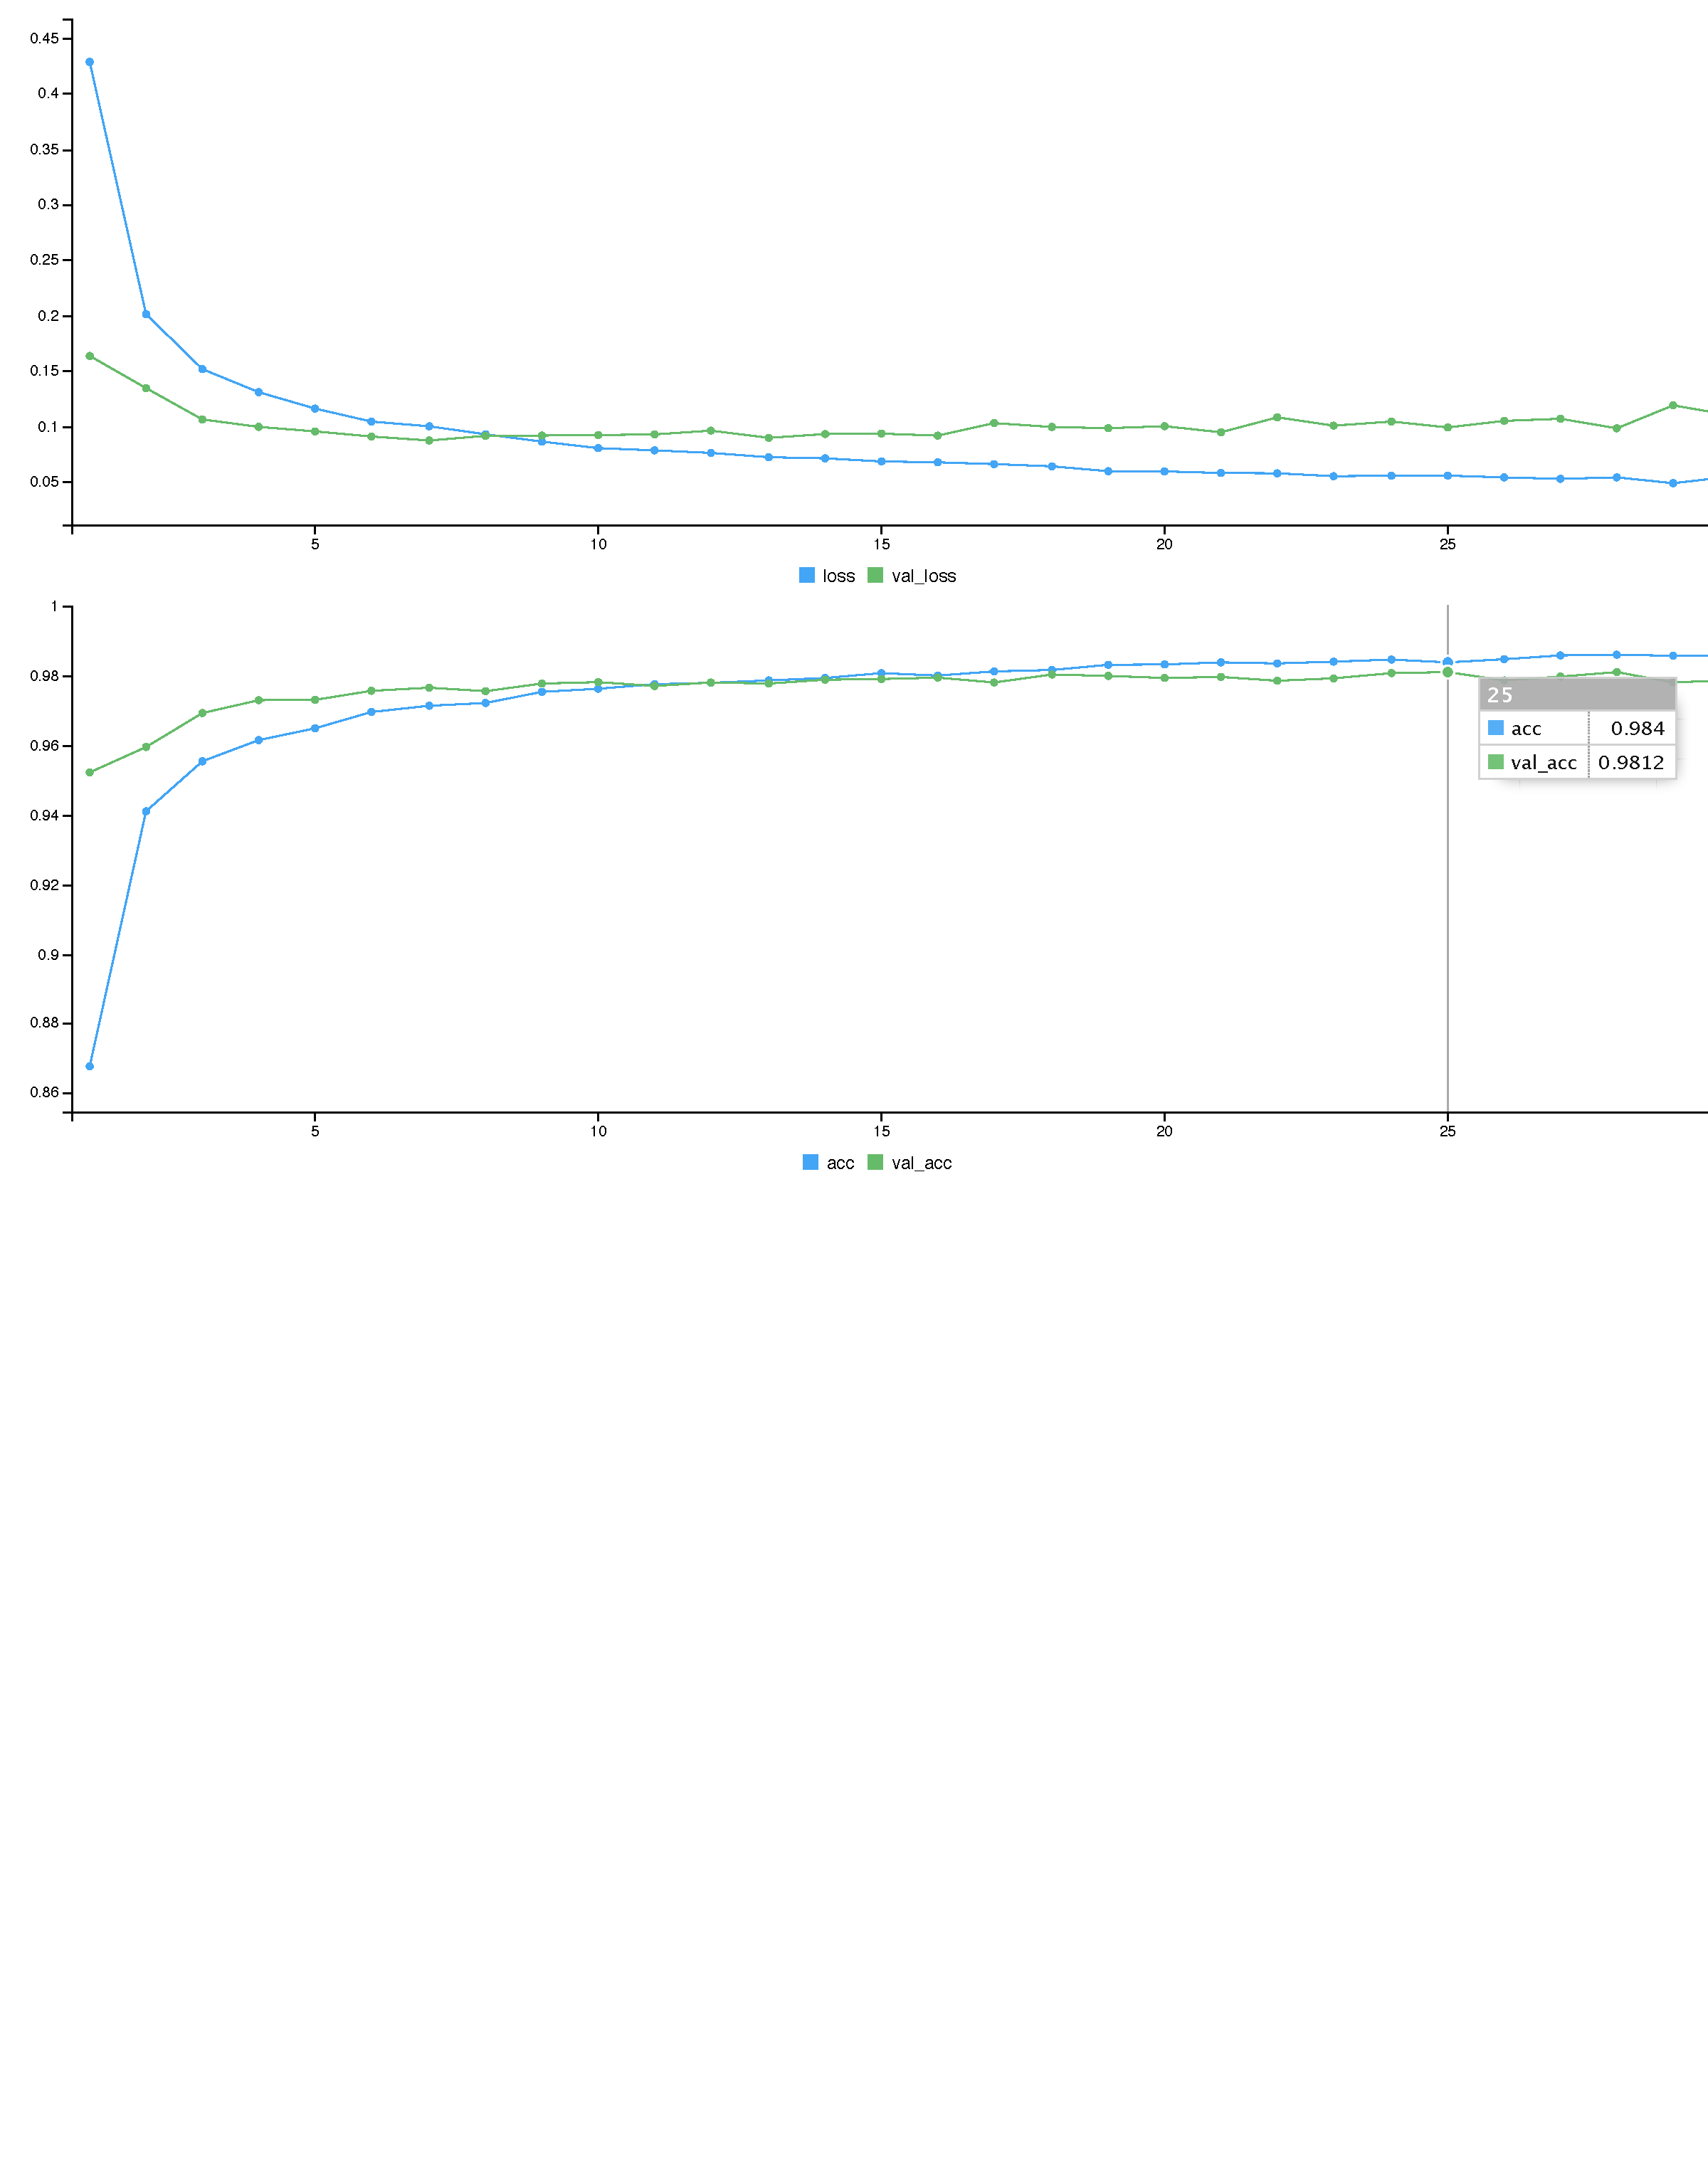
\includegraphics[width=4cm, height=4cm]{2D_FCN_mnist.pdf}
        \column{0.4\textwidth}
            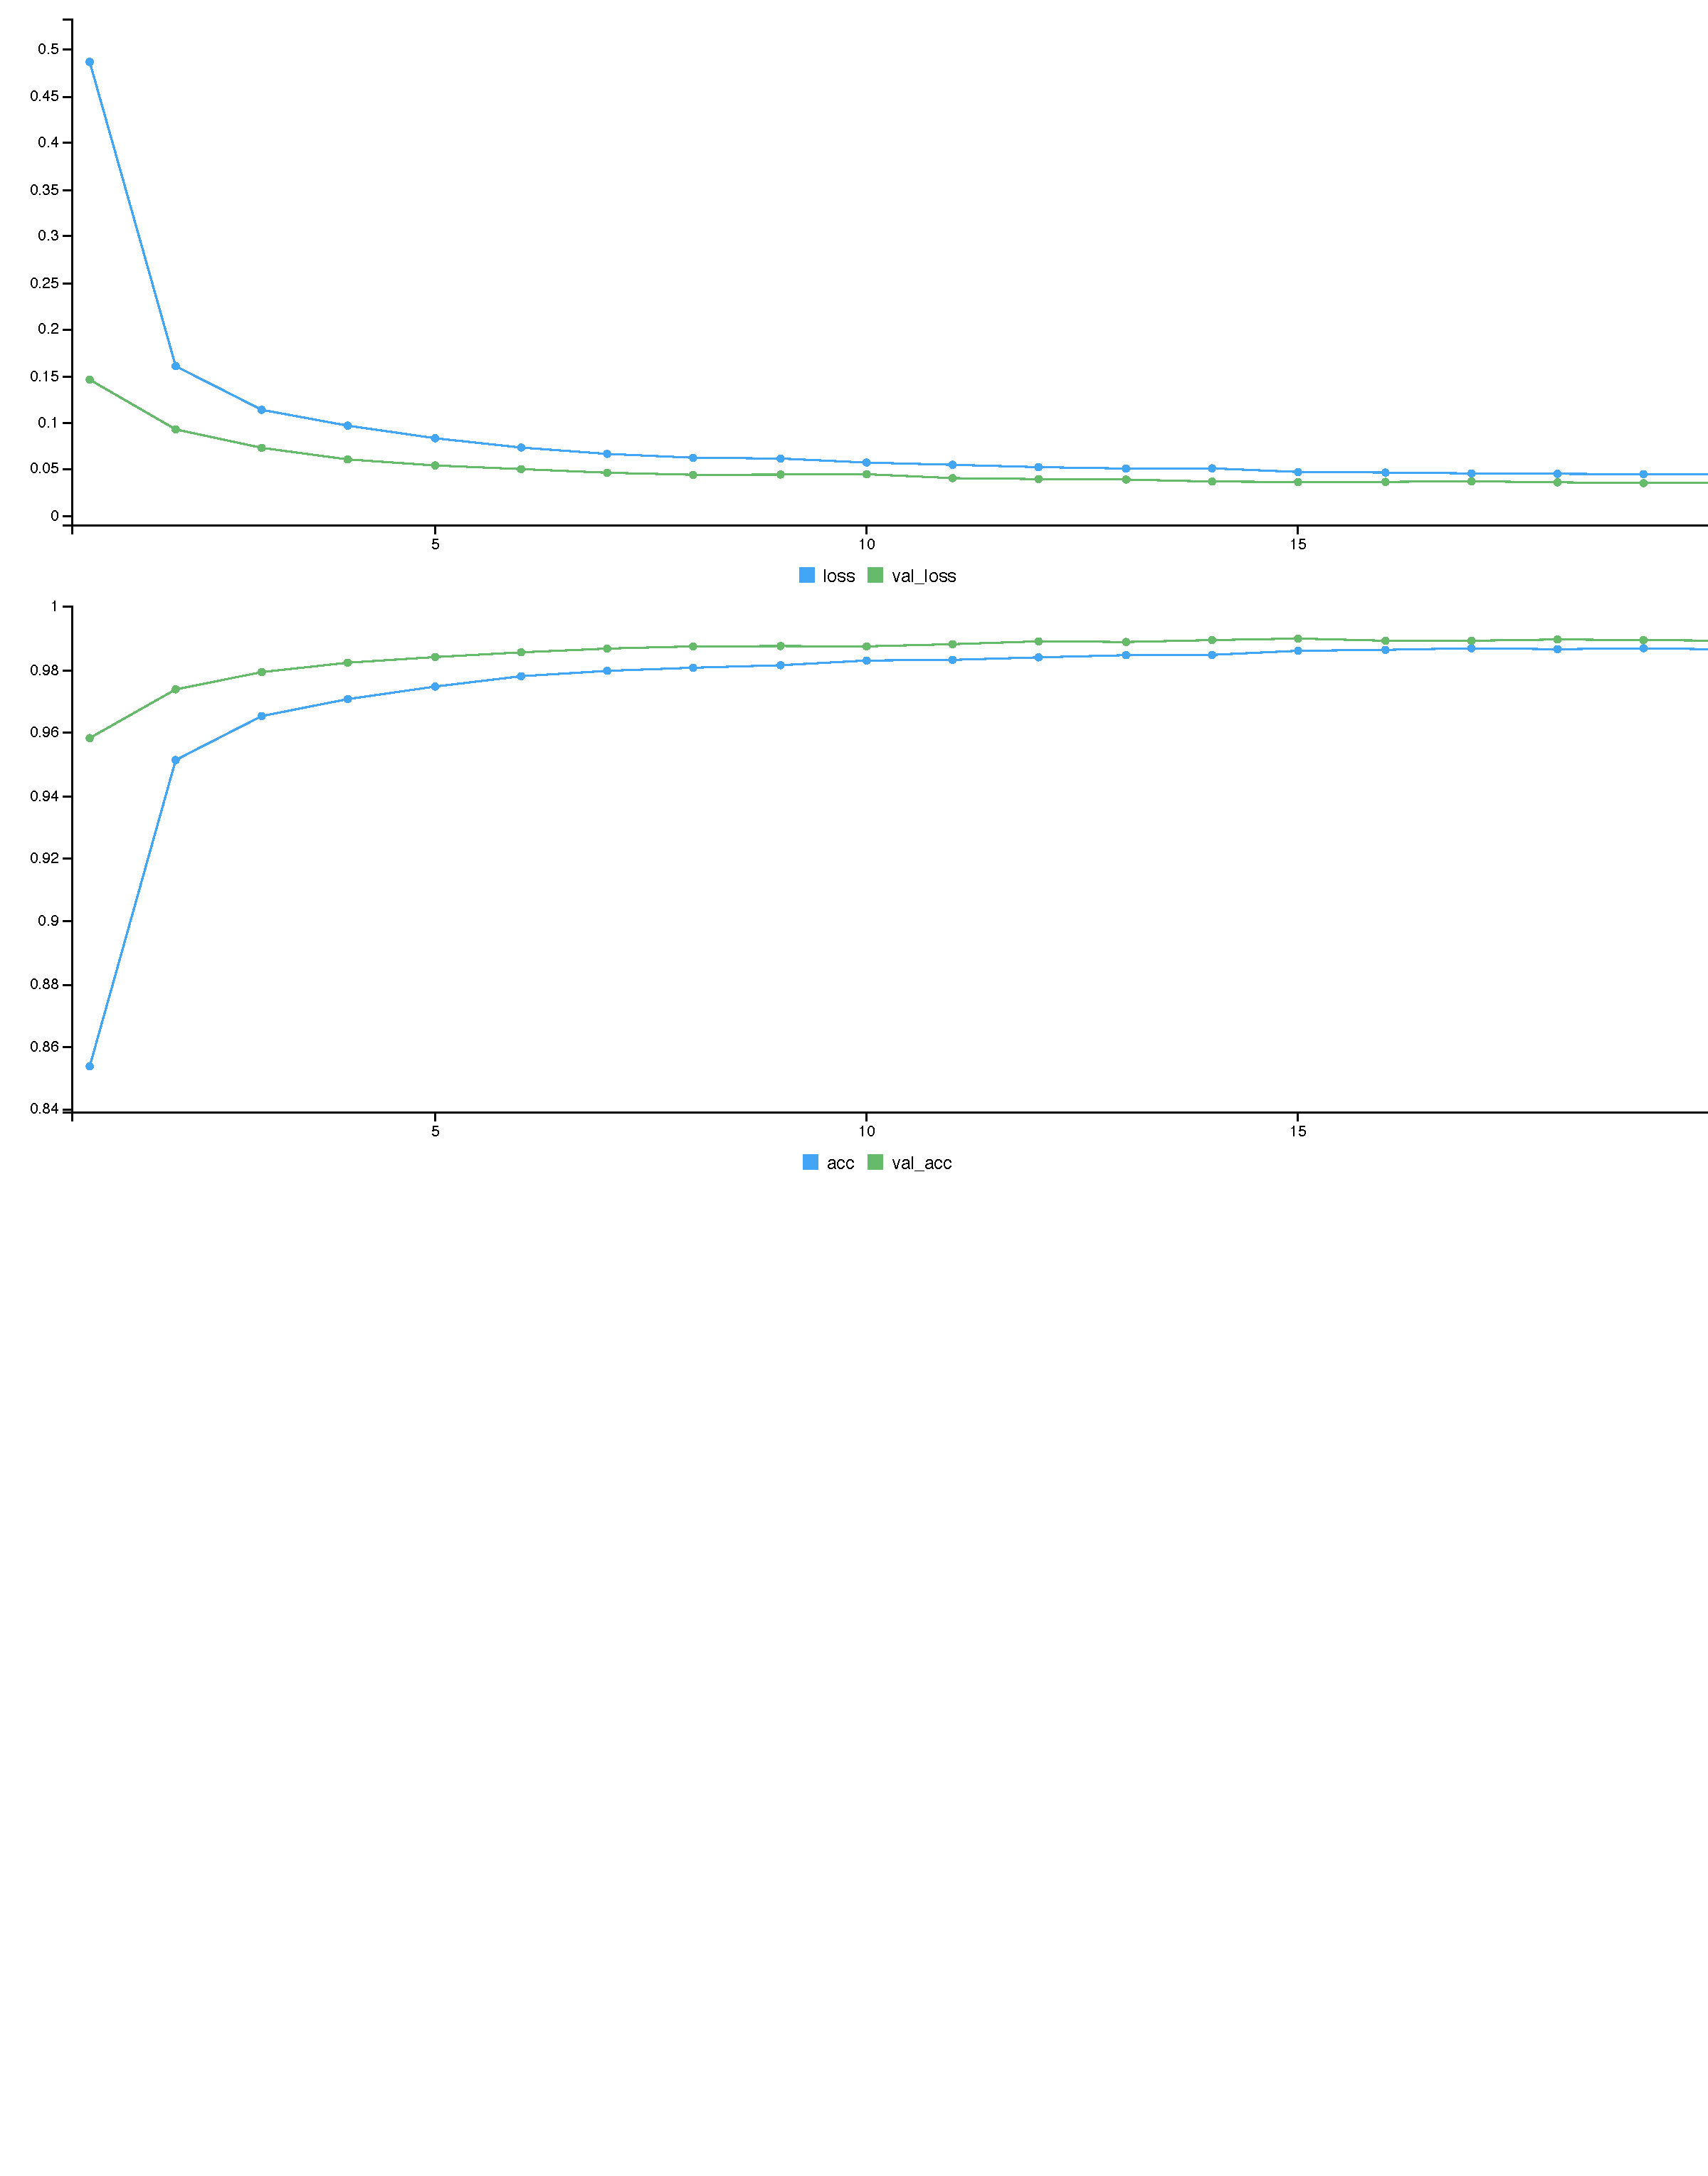
\includegraphics[width=4cm, height=4cm]{2D_CNN_mnist.pdf}
    \end{columns}
    \end{frame}
    
    \begin{frame}{Results}
      \framesubtitle{FCN vs CNN}
      \begin{block}
      {\small{FCN confusion matrix. acc=0.98, loss=0.105}}
      \end{block}
        \tiny{\begin{table}[]
            \begin{tabular}{lllllllllll}
             & \multicolumn{10}{c}{Reference} \\
            Prediction & 0 & 1 & 2 & 3 & 4 & 5 & 6 & 7 & 8 & 9 \\
            0 & 970 & 0 & 3 & 0 & 1 & 3 & 2 & 1 & 2 & 1 \\
            1 & 1 & 1125 & 3 & 0 & 0 & 1 & 2 & 3 & 1 & 3 \\
            2 & 1 & 3 & 1010 & 2 & 1 & 0 & 0 & 9 & 3 & 0 \\
            3 & 2 & 2 & 3 & 997 & 0 & 8 & 1 & 2 & 5 & 8 \\
            4 & 0 & 0 & 1 & 0 & 963 & 1 & 2 & 0 & 7 & 16 \\
            5 & 1 & 1 & 0 & 3 & 0 & 869 & 3 & 0 & 4 & 1 \\
            6 & 2 & 2 & 2 & 0 & 5 & 5 & 947 & 0 & 2 & 0 \\
            7 & 1 & 0 & 5 & 4 & 1 & 2 & 0 & 1007 & 3 & 8 \\
            8 & 1 & 2 & 5 & 2 & 2 & 2 & 1 & 2 & 942 & 0 \\
            9 & 1 & 0 & 0 & 2 & 9 & 1 & 0 & 4 & 5 & 972
            \end{tabular}
            \end{table}}
    \end{frame}

    \begin{frame}{Results}
      \framesubtitle{FCN vs CNN}
      \begin{block}
      {\small{CNN confusion matrix. acc=0.99, loss=0.029}}
      \end{block}
        \tiny{\begin{table}[]
            \begin{tabular}{lllllllllll}
             & \multicolumn{10}{c}{Reference} \\
            Prediction & 0 & 1 & 2 & 3 & 4 & 5 & 6 & 7 & 8 & 9 \\
            0 & 976 & 0 & 1 & 0 & 0 & 1 & 5 & 0 & 2 & 2 \\
            1 & 0 & 1127 & 0 & 0 & 0 & 0 & 2 & 0 & 0 & 1 \\
            2 & 0 & 2 & 1029 & 1 & 0 & 0 & 0 & 8 & 3 & 0 \\
            3 & 1 & 2 & 0 & 1006 & 0 & 6 & 1 & 2 & 1 & 1 \\
            4 & 0 & 0 & 0 & 0 & 970 & 0 & 1 & 0 & 1 & 3 \\
            5 & 0 & 1 & 0 & 2 & 0 & 880 & 4 & 0 & 1 & 3 \\
            6 & 1 & 0 & 0 & 0 & 0 & 3 & 944 & 0 & 0 & 0 \\
            7 & 0 & 0 & 2 & 0 & 0 & 0 & 0 & 1014 & 1 & 2 \\
            8 & 2 & 3 & 0 & 1 & 3 & 0 & 1 & 1 & 961 & 2 \\
            9 & 0 & 0 & 0 & 0 & 9 & 2 & 0 & 3 & 4 & 995
            \end{tabular}
            \end{table}}
    \end{frame}
    
    \begin{frame}{Results}
      \begin{block}{Teachable moments.}
      \end{block}
      \begin{columns}[onlytextwidth]
        \column{.4\textwidth}
            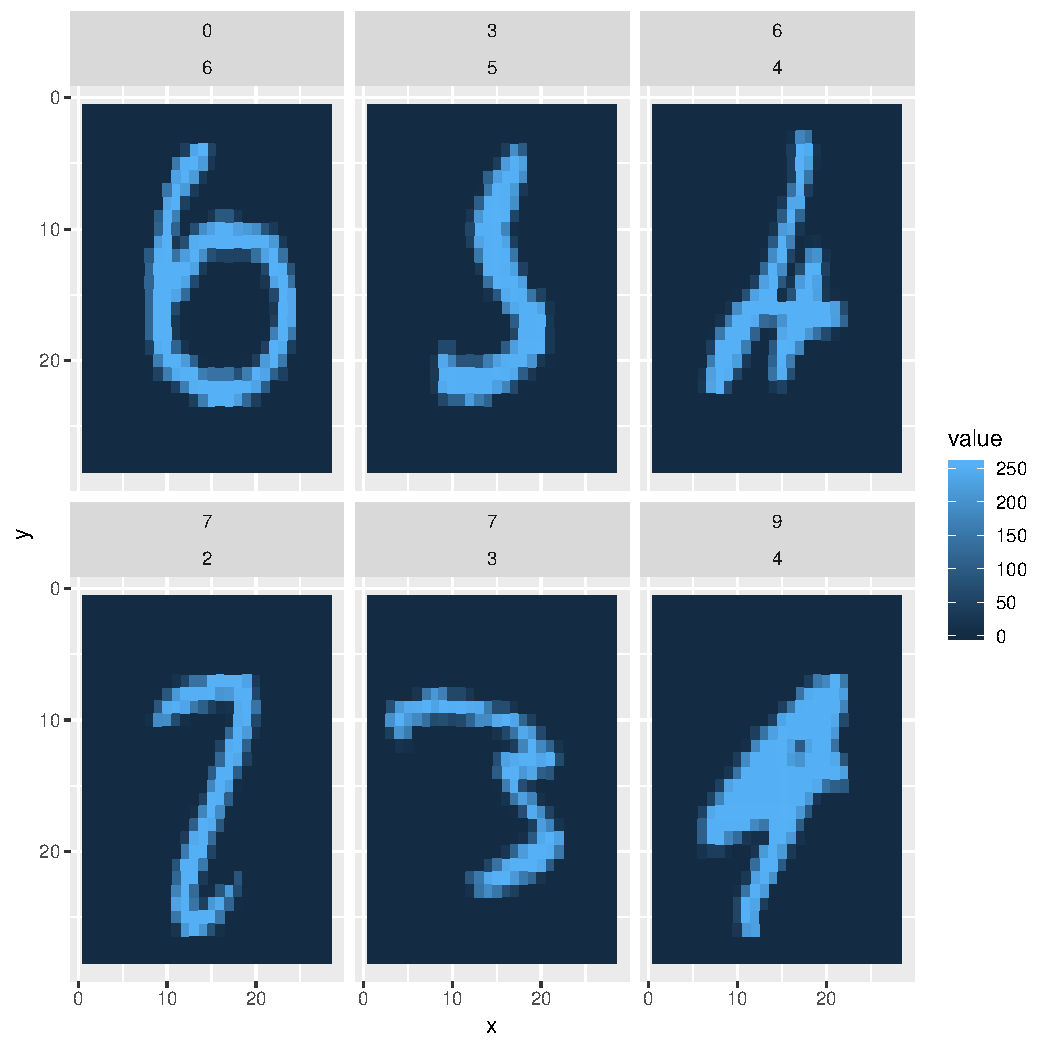
\includegraphics[width=4cm, height=4cm]{bad_pred.pdf}
        \column{.4\textwidth}
            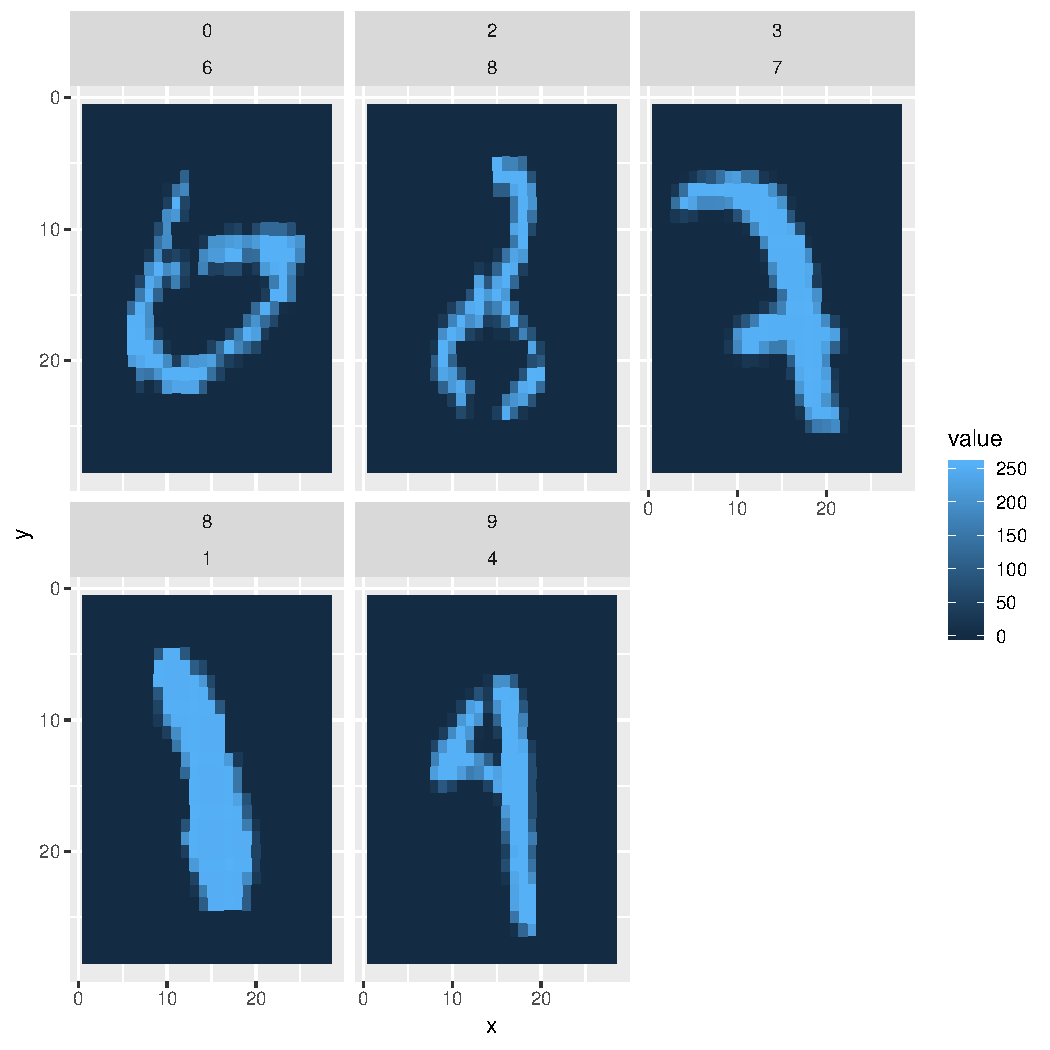
\includegraphics[width=4cm, height=4cm]{bad_pred2.pdf}
    \end{columns}
    \end{frame}

    
        \begin{frame}{Questions?}
      \begin{block}
      {{Thank you for your time...}}
      {\begin{flushright}and attention.\end{flushright}}
      \end{block}
    \end{frame}

  \end{darkframes}
\end{document}
